\documentclass[border=10pt]{standalone}
\usepackage{tikz}
\usetikzlibrary{arrows.meta}
\begin{document}
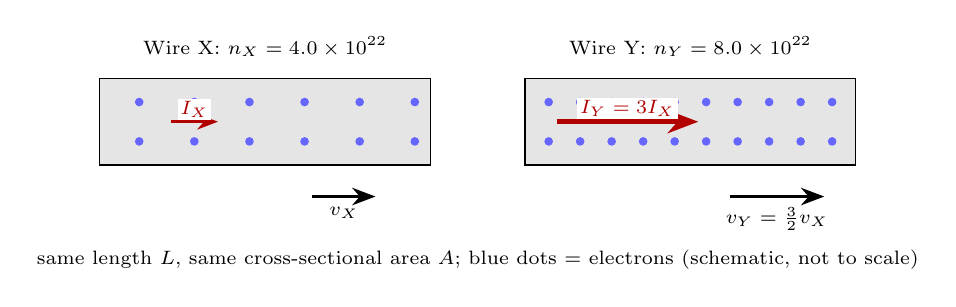
\begin{tikzpicture}[>=Stealth, scale=1.0, every node/.style={font=\scriptsize}]

% ---- Wire X ----
\fill[gray!20] (-4.8,-0.55) rectangle (-0.6,0.55);
\draw (-4.8,-0.55) rectangle (-0.6,0.55);
% electron dots: fewer (density 4.0e22)
\foreach \x in {-4.3,-3.6,-2.9,-2.2,-1.5,-0.8} {
  \foreach \y in {-0.25,0.25} {
    \fill[blue!60] (\x,\y) circle (0.055);
  }
}
% current arrow (length 0.6)
\draw[->, line width=1pt, red!70!black] (-3.9,0) -- (-3.3,0) node[midway,above,fill=white,inner sep=1pt] {$I_X$};
% drift velocity arrow (length 0.8)
\draw[->, line width=1.2pt] (-2.1,-0.95) -- (-1.3,-0.95) node[midway,below] {$v_X$};
\node at (-2.7,0.95) {Wire X: $n_X=4.0\times10^{22}$};

% ---- Wire Y ----
\fill[gray!20] (0.6,-0.55) rectangle (4.8,0.55);
\draw (0.6,-0.55) rectangle (4.8,0.55);
% electron dots: twice as many (density 8.0e22)
\foreach \x in {0.9,1.3,1.7,2.1,2.5,2.9,3.3,3.7,4.1,4.5} {
  \foreach \y in {-0.25,0.25} {
    \fill[blue!60] (\x,\y) circle (0.055);
  }
}
% current arrow (length 1.8 = 3x)
\draw[->, line width=1.8pt, red!70!black] (1.0,0) -- (2.8,0) node[midway,above,fill=white,inner sep=1pt] {$I_Y=3I_X$};
% drift velocity arrow (length 1.2 = 1.5x)
\draw[->, line width=1.2pt] (3.2,-0.95) -- (4.4,-0.95) node[midway,below] {$v_Y=\frac{3}{2} v_X$};
\node at (2.7,0.95) {Wire Y: $n_Y=8.0\times10^{22}$};

% ---- shared annotation ----
\node at (0,-1.75) {same length $L$, same cross-sectional area $A$; blue dots = electrons (schematic, not to scale)};
\end{tikzpicture}
\end{document}
